\documentclass[a4paper,12pt]{article}%
\usepackage[T1]{fontenc}%
\usepackage[utf8]{inputenc}%
\usepackage{lmodern}%
\usepackage{textcomp}%
\usepackage{lastpage}%
\usepackage{graphicx}%
%

\usepackage[left=1.5cm,right=1.5cm,top=2cm,bottom=2cm]{geometry}
\usepackage{setspace}
\onehalfspacing
\usepackage[portuguese]{babel}
\usepackage{caption}
\usepackage{amsmath}
\usepackage{cals, ragged2e}
\usepackage{breqn}
\usepackage{pdflscape}
\usepackage{multicol}
\usepackage[colorlinks=true,linkcolor=black,anchorcolor=black,citecolor=black,filecolor=black,menucolor=black,runcolor=black,urlcolor=black]{hyperref}
\usepackage{float}
\usepackage{gensymb}
\usepackage{fancyhdr}
\pagestyle{fancy}
\fancyhf{}
\rhead{
\includegraphics[width=0.05\textwidth]{figs/logo.png}}
\lhead{Structures Explained}
\cfoot{\thepage}
\renewcommand{\footrulewidth}{0.4pt}
\usepackage[scaled=1]{helvet}
\renewcommand{\familydefault}{\sfdefault}
%
%
\begin{document}%
\normalsize%

            \begin{titlepage}
            
            \newcommand{\HRule}{\rule{\linewidth}{0.5mm}}
            
            \center
            
            
\includegraphics[width=0.75\textwidth]{figs/logo.png}\\[1cm]
            \vspace{\fill}
            {\LARGE Structures Explained\\ Resolução da Seção Transversal}\\[1.5cm]
            
            \HRule \\[0.6cm]
            
                 \large\textbf{Laboratório AeroTech}\\[0.5cm]
                 \large\textbf{Departamento de Engenharia Aeronáutica}\\[0.5cm]
                 \textsc{\Large Universidade de São Paulo}\\[0.5cm]
                 
             \HRule \\[1.5cm]            
            
             \vfill
        
             \end{titlepage}
        
             \newpage
             %
\section{Subdividir a geometria da seção transversal em formas geométricas (subáreas) de propriedades conhecidas}%
\label{sec:Subdividirageometriadaseotransversalemformasgeomtricas(subreas)depropriedadesconhecidas}%


\begin{figure}[H]%
\centering%
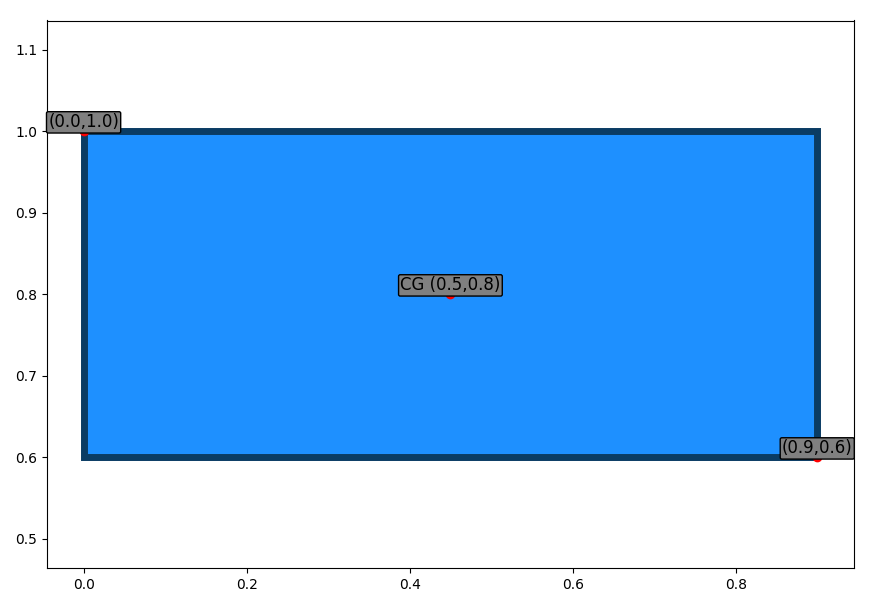
\includegraphics[width=500px]{figs/sectransv}%
\caption{\label{fig:estrutura} Estrutura com subáreas contornadas de preto}%
\end{figure}

%
\section{Calcular os momentos estáticos em relação ao eixo de interesse}%
\label{sec:Calcularosmomentosestticosemrelaoaoeixodeinteresse}%
\subsection{Cálculo do momento estático em relação ao eixo X:}%
\label{subsec:ClculodomomentoestticoemrelaoaoeixoX}%
\begin{dmath*}%
Ms_{x_{total}} = \sum{Ms_x} \\%
\end{dmath*}%
\begin{dmath*}%
Ms_x = Área_{(subárea)} \cdot \overline{Y} \\%
\end{dmath*}%
\begin{dmath*}%
Ms_{x_{total}} = 5.0 \cdot 50 + 50 \cdot 5.0%
\end{dmath*}%
\begin{dmath*}%
Ms_{x_{total}} = 500.0$ $m^3%
\end{dmath*}

%
\subsection{Cálculo do momento estático em relação ao eixo Y:}%
\label{subsec:ClculodomomentoestticoemrelaoaoeixoY}%
\begin{dmath*}%
Ms_{y_{total}} = \sum{Ms_y} \\%
\end{dmath*}%
\begin{dmath*}%
Ms_y = Area_{(subárea)} \cdot \overline{X} \\%
\end{dmath*}%
\begin{dmath*}%
Ms_{y_{total}} = 2.5 \cdot 50 + 50 \cdot 7.5%
\end{dmath*}%
\begin{dmath*}%
Ms_{y_{total}} = 500.0$ $m^3%
\end{dmath*}

%
\section{Calcular os centroides em relação ao eixo de interesse}%
\label{sec:Calcularoscentroidesemrelaoaoeixodeinteresse}%
\subsection{Cálculo do centroide em relação ao eixo X:}%
\label{subsec:ClculodocentroideemrelaoaoeixoX}%
\begin{dmath*}%
X_{cg} = \frac{Ms_y}{A_{total}}%
\end{dmath*}%
\begin{dmath*}%
X_{cg} = \frac{2.5 \cdot 50 + 50 \cdot 7.5}{50 + 50}$ $m%
\end{dmath*}%
\begin{dmath*}%
X_{cg} = 5.0$ $m%
\end{dmath*}

%
\subsection{Cálculo do centroide em relação ao eixo Y:}%
\label{subsec:ClculodocentroideemrelaoaoeixoY}%
\begin{dmath*}%
Y_{cg} = \frac{Ms_x}{A_{total}}%
\end{dmath*}%
\begin{dmath*}%
Y_{cg} = \frac{5.0 \cdot 50 + 50 \cdot 5.0}{50 + 50}$ $m%
\end{dmath*}%
\begin{dmath*}%
Y_{cg} = 5.0$ $m%
\end{dmath*}

%
\section{Calcular os momentos de inércia em relação aos eixos de interesse}%
\label{sec:Calcularosmomentosdeinrciaemrelaoaoseixosdeinteresse}%
Quando necessário (ou, na dúvida, sempre), aplicar o teorema dos eixos paralelos \\%
Teorema dos eixos paralelos: I' = I + A * d² \\%
\subsection{Cálculo do Momento de Inércia em relação a X:}%
\label{subsec:ClculodoMomentodeInrciaemrelaoaX}%
\begin{dmath*}%
I_{x_{total}} = \sum{I_x}%
\end{dmath*}%
\begin{dmath*}%
I_{x_{(retângulos)}} = \frac{base \cdot altura^3}{12}%
\end{dmath*}%
\begin{dmath*}%
I_{x_{total}} = \frac{5 \cdot 10^{3}}{12} + \frac{5 \cdot 10^{3}}{12}%
\end{dmath*}%
\begin{dmath*}%
I_{x_{total}} = 2500/3$ $m^4%
\end{dmath*}

%
\subsection{Cálculo do Momento de Inércia em relação a Y:}%
\label{subsec:ClculodoMomentodeInrciaemrelaoaY}%
\begin{dmath*}%
I_{y_{total}} = \sum{Iy}%
\end{dmath*}%
\begin{dmath*}%
I_{y_{(retângulos)}} = \frac{base^3 \cdot altura}{12}%
\end{dmath*}%
\begin{dmath*}%
I_{y_{total}} = 5^{3} \cdot 10 \frac{1}{12} + 5^{3} \cdot 10 \frac{1}{12} + 50 \left(5.0 - 2.5\right)^{2} + 50 \left(5.0 - 7.5\right)^{2}%
\end{dmath*}%
\begin{dmath*}%
I_{y_{total}} = 833.33$ $m^4%
\end{dmath*}

%
\section{Cálculo da Tensão Normal}%
\label{sec:ClculodaTensoNormal}%
\subsection{Fórmula da Tensão Normal}%
\label{subsec:FrmuladaTensoNormal}%
\begin{dmath*}%
T_{normal} = \frac{N}{A} - \frac{My}{Iy} \cdot z - \frac{Mz}{Iz} \cdot y%
\end{dmath*}

%
\subsection{Cálculo para N = 10 N, My = 500.0 Nm, Mz = 500.0 Nm, y = 1 m, z = z m}%
\label{subsec:ClculoparaN=10N,My=500.0Nm,Mz=500.0Nm,y=1m,z=zm}%
\subsubsection{Cálculo da Tensão Normal}%
\label{ssubsec:ClculodaTensoNormal}%
\begin{dmath*}%
T_{normal} =- \frac{500.0 z}{833.33} - 500.0 \frac{1}{2500} \frac{1}{3} \cdot 1 + \frac{10}{100}%
\end{dmath*}%
\begin{dmath*}%
T_{normal} =0.03 - 0.6*z$ $Pa%
\end{dmath*}

%
\section{Cálculo da Linha Neutra}%
\label{sec:ClculodaLinhaNeutra}%
\subsection{Fórmula da Linha Neutra}%
\label{subsec:FrmuladaLinhaNeutra}%
A linha neutra se encontra onde a Tensão Normal é 0, portanto para encontrar a posição da linha neutra (y) substituímos T por 0.%
\begin{dmath*}%
0 = \frac{N}{A} - \frac{My}{Iy} \cdot z - \frac{Mz}{Iz} \cdot y%
\end{dmath*}

%
\subsection{Cálculo para N = 10 N, My = 500.0 Nm, Mz = 500.0 Nm, y = 1 m, z = z m}%
\label{subsec:ClculoparaN=10N,My=500.0Nm,Mz=500.0Nm,y=1m,z=zm}%
\subsubsection{Cálculo da Linha Neutra}%
\label{ssubsec:ClculodaLinhaNeutra}%
\begin{dmath*}%
0 = - \frac{500.0 z}{833.33} - 500.0 \frac{1}{2500} \frac{1}{3} \cdot 1 + \frac{10}{100}%
\end{dmath*}%
\begin{dmath*}%
z = 0.06%
\end{dmath*}

%
\section{Calcular o Momento Estático no corte}%
\label{sec:CalcularoMomentoEstticonocorte}%
\subsection{Fórmula do Momento Estático para corte sobre a subárea}%
\label{subsec:FrmuladoMomentoEstticoparacortesobreasubrea}%
\begin{dmath*}%
M_{estático_{corte}} = Área_{subárea} \cdot (centroide_{subárea} - centroide_{figura}) %
\end{dmath*}

%
\subsection{Fórmula do Momento Estático para corte acima ou abaixo da subárea}%
\label{subsec:FrmuladoMomentoEstticoparacorteacimaouabaixodasubrea}%
\begin{dmath*}%
M_{estático_{corte}} = (\frac{altura}{2} + centroide_{subárea}- corte_y) \cdot base \cdot ((\frac{altura}{2} + centroide_{subárea} - corte_y) \cdot 0.5 + corte_y - centroide_{figura}) %
\end{dmath*}

%
\subsection{Calcular o Momento Estático no corte}%
\label{subsec:CalcularoMomentoEstticonocorte}%
\begin{dmath*}%
M_{estático_{corte}} =5 \left(\left(-1\right) 5 + \frac{10}{2} + 5.0\right) \left(\left(-1\right) 5.0 + \left(\left(-1\right) 5 + \frac{10}{2} + 5.0\right) 0.5 + 5\right) + \left(\left(-1\right) 5 + \frac{10}{2} + 5.0\right) 5 \left(\left(-1\right) 5.0 + \left(\left(-1\right) 5 + \frac{10}{2} + 5.0\right) 0.5 + 5\right)%
\end{dmath*}%
\begin{dmath*}%
M_{estático_{corte}} =125.0$ $m^3%
\end{dmath*}

%
\section{Calcular o Fluxo de Cisalhamento}%
\label{sec:CalcularoFluxodeCisalhamento}%
\subsection{Fórmula do Fluxo de Cisalhamento}%
\label{subsec:FrmuladoFluxodeCisalhamento}%
\begin{dmath*}%
f_{cisalhamento} = \frac{V \cdot Q}{I_x}%
\end{dmath*}

%
\subsection{Cálculo para V = 10 N, Q = 45.0 m\textsuperscript{3}, I\textsubscript{x} = 2500/3 m\textsuperscript{4}}%
\label{subsec:ClculoparaV=10N,Q=45.0mtextsuperscript3,Itextsubscriptx=2500/3mtextsuperscript4}%
\begin{dmath*}%
f_{cisalhamento} =10 \cdot 45.0 \frac{1}{2500 \frac{1}{3}}%
\end{dmath*}%
\begin{dmath*}%
f_{cisalhamento} =0.54$ $\frac{N}{m}%
\end{dmath*}

%
\section{Calcular a Tensão de Cisalhamento}%
\label{sec:CalcularaTensodeCisalhamento}%
\subsection{Fórmula da Tensão de Cisalhamento}%
\label{subsec:FrmuladaTensodeCisalhamento}%
\begin{dmath*}%
T_{cisalhamento} = \frac{V \cdot Q}{I_x \cdot t}%
\end{dmath*}

%
\subsection{Cálculo para V = 10 N, Q = 125.0 m\textsuperscript{3}, I\textsubscript{x} = 2500/3 m\textsuperscript{4}, t = 10 m}%
\label{subsec:ClculoparaV=10N,Q=125.0mtextsuperscript3,Itextsubscriptx=2500/3mtextsuperscript4,t=10m}%
\begin{dmath*}%
T_{cisalhamento} =10 \cdot 125.0 \frac{1}{10 \cdot 2500 \frac{1}{3}}%
\end{dmath*}%
\begin{dmath*}%
T_{cisalhamento} =0.15$ $Pa%
\end{dmath*}

%
\end{document}